% Chapter 1

\chapter{Preliminary} % Main chapter title

\label{Chapter3} % For referencing the chapter elsewhere, use \ref{Chapter1} 


This chapter is dedicated to the two main tools that will be widely used in this manuscript. To avoid redundancy and repetitive explanations, we propose defining Polarization in Section \ref{Polar_explain} and Deep Learning in Section \ref{DL_explain}. Thus, when general principles are needed for the understanding of the work, this chapter will serve as a reference.
%----------------------------------------------------------------------------------------

% Define some commands to keep the formatting separated from the content 


%----------------------------------------------------------------------------------------

\section{Polarimetry}\label{Polar_explain}

This section will be dedicated to polarimetry and will provide a general introduction to the field. We propose to describe this modality by defining it in three aspects. First, Section \ref{gdpola} introduce the general concept of polarization. Then, Section \ref{particularsensor} will take the sensor angle to discuss the properties specific to polarimetric imaging. Finally, in Section \ref{exploitdata}, we will discuss the usual exploitation methods of this particular data.


\subsection{General Principles}\label{gdpola}

Polarimetry \cite{collett2005field} is a particular modality that acquires the polarization state of objects in a scene. Briefly, polarization is a property that, in the case of image acquisition, concerns light. It is composed of two perpendicular fields called electric field $\vec{E}$ and magnetic field $\vec{B}$ that oscillate along the wave reflected to the sensor. A polarized wave is said to be elliptical but is ordinarily considered as the sum of linear and circular components.
In general, in mobile acquisition systems, only the linear polarization is acquired since the circular polarization requires the mounting of a quarter wave plate.
It is possible to observe polarized light in nature with sunlight or observation of multiple non-natural light sources. A notable property of polarization is that if a light wave hits a surface and is reflected, then the wave becomes partially polarized. This property is particularly important since, unlike conventional modalities that focus on colors or textures, polarimetry focuses on light behavior in relation to surfaces.

Consequently, it is possible to affirm that polarimetry allows the acquisition of changes in the state of light\cite{wolff1995polarization}. In addition, many principles are inspired or derived from Fresnel's equations \cite{fresnel1868oeuvres}. This link is attributed to the close relationship between polarization and reflection of light. Therefore, it is notable that polarization has the potential capacity to infer, by light behavior, the properties of surfaces (i.e. refractive index, surface normals, etc.).



\subsection{A Particular Sensor}\label{particularsensor}

The sensor allowing the acquisition of such data is particular.
Indeed, it could be compared to RGB if we consider the Bayer matrix. As shown in Figure \ref{fig:sensor}, a polarimetric camera has a microgrid of polarizers that allow the acquisition of polarization.

\begin{figure}[h]
	\centering
	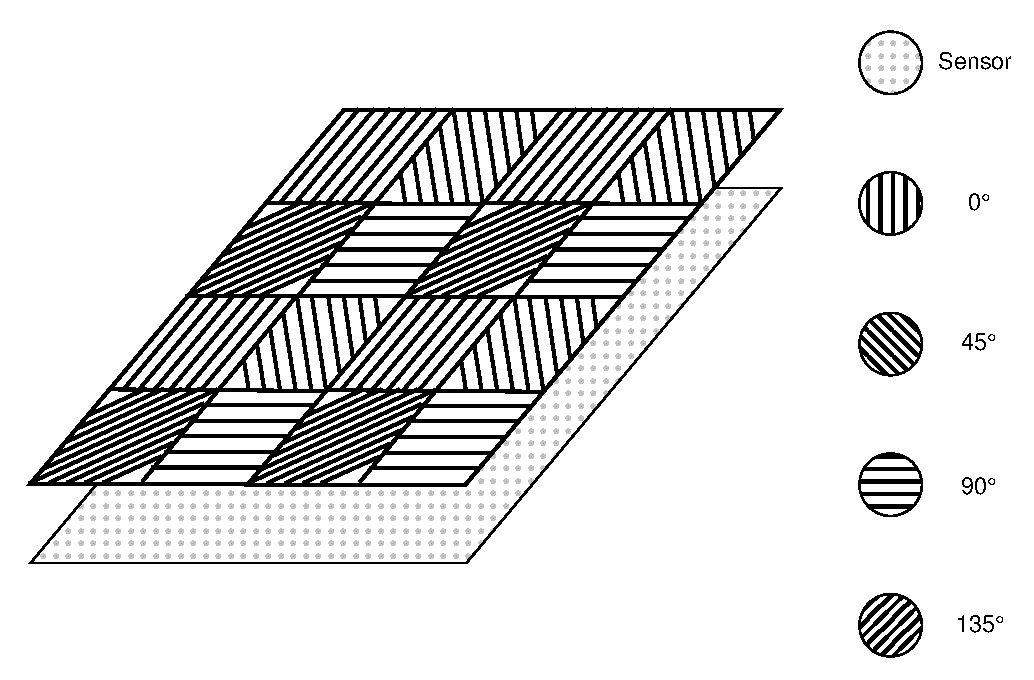
\includegraphics[width=0.8\linewidth]{Figures/Preliminary/sensor}
	\caption{Illustration of a DoFP polarization sensor micro-grid.}
	\label{fig:sensor}
\end{figure}

It is then possible to observe a multitude of mini polarizers with four different orientations affixed to the sensor. This technology is called Division of Focal Plane (DoFP).
Before the arrival of this technology, the cameras required a mechanical action to rotate the polarizers in front of the camera. Since then, with the DoFP, it is possible to acquire all the necessary information in a single shot. Hence, the sensors could be embedded to make dynamic acquisitions.
Standardly, there are four angles $\{0,45,90,135\}$ allowing calculations which will be discussed below.
These different angles allow discriminating the components of the light and thus to separate the waves. As schematized in Figure \ref{extract}, thanks to these different orientations, the light can be filtered.

\begin{figure}{h}
	\centering
	\colorlet{crystal}{gray}
	
	\def\zangle{-20}
	\def\xangle{20}
	
	\begin{tikzpicture}[x=(\xangle:0.75cm), y=(90:1cm), z=(\zangle:1.5cm),
	>=stealth, line cap=round, line join=round,
	lines/.style={gray!70, thick}, 
	axis/.style={black, thick},
	plate/.style={fill, opacity=0.875},
	markers/.style={darkgray!80, thick},
	markerss/.style={black!30, thick}]
	
	
	
	
	\begin{scope}[shift={(0,0,3.125)}]
	
	\node [yslant=tan(\zangle), above=0.25cm, align=center,font=\footnotesize] at 
	(1,1,1.5){Linearly Polarized Light};
	
	\begin{scope}[xscale=1.5, yscale=1.5]
	\path [crystal!25, plate] 
	(-1,-1,0) -- (-1,1,0) -- (1,1,0) -- (1,-1,0) -- cycle;
	\path [crystal!50, plate] 
	(-1,-1,0) -- (-1,-1,-0.125) -- (-1,1,-0.125) -- (-1,1, 0) -- cycle;
	\path [crystal!75, plate] 
	(-1,1,0) -- (-1,1,-0.125) -- (1,1,-0.125) -- (1,1, 0) -- cycle;
	\node [yslant=tan(\xangle), text=crystal!50, below, font=\small] at 
	(-1.125,-1,0){Sensor};
	\end{scope}
	
	
	\draw [markers] (0,1) -- (0,-1) (-0.5,0) -- (0.5,0);
	
	\draw [axis] (0,0,0) -- (0,0,3);
	
	\foreach \k [evaluate={%
		\i=\k*5.625; \j=\i>0 ? \i-5.625 : 0; 
		\a=90-\i; 
		\b=90-\j; 
		\c=int(mod(\k,4)==0 && sin \a != 0); 
		\d=int(\k+1/4);}] in {0,...,192}{
		\ifodd\d
		\ifnum\c=1
		\draw [->,opacity=0.3] (0,0,\i/360) -- ++(sin \a, sin \a, 0);
		\fi
		\draw [thick, red!80] (sin \a, sin \a, \i/360) -- (sin \b, sin \b, \j/360);
		\else
		\draw [thick, red!80] (sin \a, sin \a, \i/360) -- (sin \b, sin \b, \j/360);
		\ifnum\c=1
		\draw [->,opacity=0.3] (0,0,\i/360) -- ++(sin \a, sin \a, 0);
		\fi
		\fi
	}
	\end{scope}
	
	\begin{scope}[shift={(0,0,6.125)}]
	
	\node [yslant=tan(\zangle), above=0.25cm, align=center,font=\footnotesize] at 
	(1,1,1.5){Unpolarized Light};
	
	\begin{scope}[xscale=1.5, yscale=1.5]
	\path [crystal!25, plate] 
	(-1,-1,0) -- (-1,1,0) -- (1,1,0) -- (1,-1, 0) -- cycle;
	\path [crystal!50, plate] 
	(-1,-1,0) -- (-1,-1,-0.0625) -- (-1,1,-0.0625) -- (-1,1, 0) -- 
	cycle;
	\path [crystal!75, plate] 
	(-1,1,0) -- (-1,1,-0.0625) -- (1,1,-0.0625) -- (1,1, 0) -- cycle;
	\node [yslant=tan(\xangle), text=crystal!50, below, font=\small] at 
	(-1,-1,0){45$^\circ$ Linear Polarizer};
	\end{scope}
	
	
	\draw [markerss] (-1.25,0.75) -- (-0.75,1.25);
	
	\draw [markerss] (-1.25,0.25) -- (-0.25,1.25);
	
	\draw [markerss] (-1.25,-0.25) -- (0.25,1.25);
	
	\draw [markerss] (-1.25,-0.75) -- (0.75,1.25);
	%up
	\draw [markerss] (-1.25,-1.25) -- (1.25,1.25);
	%down
	\draw [markerss] (-0.75,-1.25) -- (1.25,0.75);
	
	\draw [markerss] (-0.25,-1.25) -- (1.25,0.25);
	
	\draw [markerss] (0.25,-1.25) -- (1.25,-0.25);
	
	\draw [markerss] (0.75,-1.25) -- (1.25,-0.75);
	
	
	\foreach \k [evaluate={%
		\i=\k*5.625; \j=\i>0 ? \i-5.625 : 0; 
		\a=90-\i; 
		\b=90-\j; 
		\c=int(mod(\k,4)==0 && sin \a != 0); 
		\d=int(\k+1/4);}] in {0,...,192}{
		\ifodd\d
		\ifnum\c=1
		\draw [->,opacity=0.3] (0,0,\i/360) -- ++(sin \a, sin \a, 0);
		\fi
		\draw [thick,red!80] (sin \a, sin \a, \i/360) -- (sin \b, sin \b, \j/360);
		\else
		\draw [thick,red!80] (sin \a, sin \a, \i/360) -- (sin \b, sin \b, \j/360);
		\ifnum\c=1
		\draw [->,opacity=0.3] (0,0,\i/360) -- ++(sin \a, sin \a, 0);
		\fi
		\fi
	}
	
	\foreach \k [evaluate={%
		\i=\k*5.625; \j=\i>0 ? \i-5.625 : 0; 
		\a=90-\i; 
		\b=90-\j; 
		\c=int(mod(\k,4)==0 && cos \a != 0); 
		\d=int(\k+1/4);}] in {0,...,192}{
		\ifodd\d
		\ifnum\c=1
		\draw [->,opacity=0.3] (0,0,\i/360) -- ++(cos \a, 0, 0);
		\fi
		\draw [thick,teal] (cos \a, 0, \i/360) -- (cos \b, 0, \j/360);
		\else
		\draw [thick,teal] (cos \a, 0, \i/360) -- (cos \b, 0, \j/360);
		\ifnum\c=1
		\draw [->,opacity=0.3] (0,0,\i/360) -- ++(cos \a, 0, 0);
		\fi
		\fi
	}
	
	\foreach \k [evaluate={%
		\i=\k*5.625; \j=\i>0 ? \i-5.625 : 0; 
		\a=90-\i; 
		\b=90-\j; 
		\c=int(mod(\k,4)==0 && sin \a != 0); 
		\d=int(\k+1/4);}] in {0,...,192}{
		\ifodd\d
		\ifnum\c=1
		\draw [->,opacity=0.3] (0,0,\i/360) -- ++(0, sin \a, 0);
		\fi
		\draw [thick,orange] (0, sin \a, \i/360) -- (0, sin \b, \j/360);
		\else
		\draw [thick,orange] (0, sin \a, \i/360) -- (0, sin \b, \j/360);
		\ifnum\c=1
		\draw [->,opacity=0.3] (0,0,\i/360) -- ++(0, sin \a, 0);
		\fi
		\fi
	}
	
	\draw [ultra thick, ->] (0,0,3.5) -- (0,0,3);
	
	\end{scope}
	
	\end{tikzpicture}
	\caption{Illustration of unpolarized light filtration through $45\deg$ linear polarizer.}\label{extract}
\end{figure}


This filtering is reproduced with the different orientations of each micro-polarizer and thus allows the acquisition of a multitude of linearly polarized light components. 
Due to this sensor architecture, each pixel is independent since the information is influenced by the polarizer. Consequently, the images of each polarizer $P_{\{0,45,95,135\}}$ is "independent" and especially sparse. As shown in Figure \ref{fig:polaexplain}, it is possible to recognize the microgrid by zooming in on an image.

\begin{figure}[h]
	\centering
	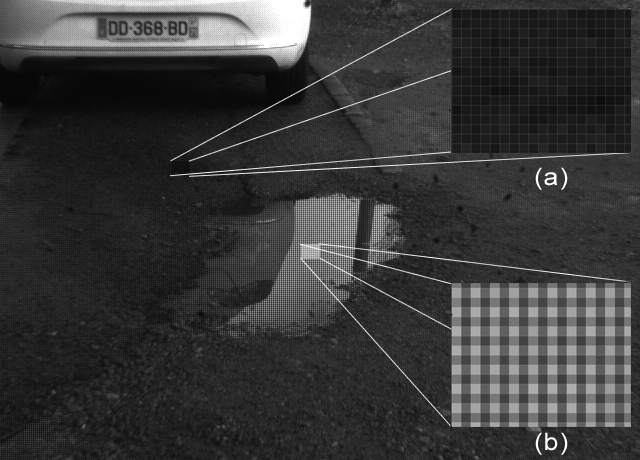
\includegraphics[width=0.6\linewidth]{Figures/VISAPP/polaexplain}
	\caption[Zoom on a polarimetric image.]{Zoom on a polarimetric image. (a) is a zoom on the non-polarized area, (b) is on a polarized area. Clearly, on a polarized surface, the micro-grid appear and reveal an intensity change according to the polarizer affected.}
	\label{fig:polaexplain}
\end{figure}

Subsequently, it is possible to identify polarized areas using this pixelization phenomenon. Indeed, when an object reflects the light, the grid appears since the intensities per polarizer are different (consequence of the filtering).


\subsection{Exploiting the Data}\label{exploitdata}


As previously stated, the images are sparse because of the sensor architecture. When the images are acquired with a low resolution sensor then this can cause a significant problem since the image size is divided by two. In addition, on a low resolution, the shapes can be changed because of the correspondence between the real world and image space. Ultimately, it is necessary that the polarizer images are dense and aligned otherwise the polarimetric information is incomplete.

To overcome this dimensionality problem, many approaches have been developed that allow the interpolation of polarimetric intensities. Principally used, Ratliff et al. \cite{ratliff2009interpolation} proposes to use a bilinear interpolation directly on the intensity images. More recently, more complex interpolation startegies have been investigated using the Newton polynomial \cite{li2019demosaicking} or the use of machine learning models based on sparse representation \cite{zhang2018sparse}.
Despite the complexity of these algorithms, the best way to overcome the image sparsity problem is to operate a high-resolution camera with smaller pixels and, above all, a more adequate real-world correspondence to image space.
The density of the polarization images is crucial to calculate the Stokes parameters \cite{stokes1851composition}.
These parameters have been designed to describe the polarization of light through a descriptive vector such as:

\begin{equation}
S = \begin{pmatrix}S_0\\S_1\\S_2\\S_3\end{pmatrix} = \begin{pmatrix}P_H + P_V\\ P_H - P_V\\ P_{45} - P_{135} \\ P_R - P_L\end{pmatrix} = \begin{pmatrix}P_0 + P_{90}\\ P_0 - P_{90}\\ P_{45} - P_{135} \\ 0\end{pmatrix} = \begin{pmatrix}I\\ Q\\ U \\ V\end{pmatrix},
\end{equation}

where $P_H$ and $P_V$ are respectively the horizontal and vertical polarization. Since we do not acquire circular polarization, $V$ and therefore $s_3$ remain null. $I$ represents the total acquired intensity whereas $U$ and $Q$ are part of $L = Q + iU$ the straight polarization intensity, being a complex number that accounts for the tilt of the polarization direction $\theta$.

\begin{figure}[h]
	\centering
	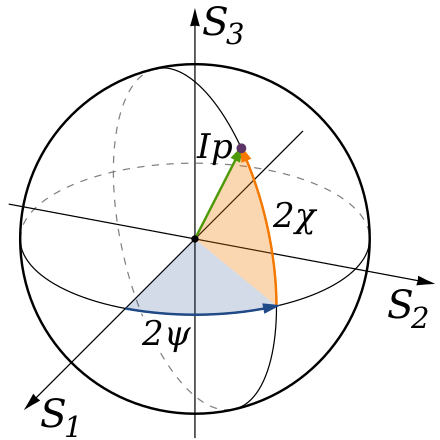
\includegraphics[width=0.3\linewidth]{Figures/Preliminary/pointcare}
	\caption{Spherical representation of Stokes vector on Poincar\'e Sphere.}
	\label{fig:pointcare}
\end{figure}

As stated in Section \ref{gdpola}, the polarization is said elliptical. Nevertheless, common representation projects the vector onto Poincar\'e sphere. Consequently, Stokes parameters can also be defined through 3 spherical coordinates $I_p$, $2\psi$ and $2\chi$ shown in Figure \ref{fig:pointcare}. Equally, the parameters are:

\begin{equation}
	\begin{cases}
	S_0 = I_p \\
	S_1 =  I_p \cos 2\psi \cos 2\chi\\
	S_2 =  I_p \sin 2\psi \cos 2\chi\\
	S_3 =  I_p \sin 2 \chi
	\end{cases},
\end{equation}

where $I_p$ is the intensity of the beam, $\psi$ and $\xi$ are defining factor for an ellipse being $\pi$ and $\frac{\pi}{2}$ invariant.
Consequently, one can define the intensity $\iota$, the angle of polarization $\alpha$ as well as the degree of polarization $\rho$ following (with no circular polarization acquired): 

\begin{equation}
\begin{cases}
\iota = S_0 =  I_p \\[8pt] 
\alpha = \frac{1}{2} \arctan \frac{S_2}{S_1}  = \psi\\[8pt] 
\rho =  \frac{\sqrt{S_1^2 + S_2^2}}{S_0}
\end{cases}.
\end{equation}

The degree $\rho$ and angle $\alpha$ of polarization are two very descriptive characteristics of polarization. $\rho$ is analogous to the polarization strength and belongs to $\left[0,1\right]$. This parameter quantify the polarization light in a wave. Therefore, a completly specular wave will record $\rho = 1$.

$\alpha \in \left[\frac{-\pi}{2}, \frac{\pi}{2}\right]$ is the angle of the electric field $\vec{E}$ projected on the image plane. In other words, the polarization angle corresponds to the orientation of the polarization with regard to the incident plane.

\subsection{Summary}

This section review the fundamental principles of polarization imaging. It showed how this modality is particular and requires a singular processing. In the same way, it is possible to realize that this information can be very useful for certain domains. Indeed, we have first stated the particularities of the acquisition of the polarization state of objects. This allowed us to establish a direct link between the surface and the light reflected by it. Next, we described the functioning of the sensors and their limits. To conclude, we have described general process making raw polarimetric images exploitable. This brief overview has, in addition to introducing the subject and establishing it, justified in large part the use of this particular information in our work.





\section{Deep Learning}\label{DL_explain}

This section will be dedicated to the main notions related to Deep Learning. The recent advances in the field of learning and the increase in computing power have allowed this sub-branch of machine learning to emerge. Moreover, the availability of data, which is crucial for this kind of greedy algorithm, has allowed to guarantee a certain viability to these models. All in all, DL has become an inner part of the computer vision field by imposing itself as a powerful processing core for many approaches.

We propose detailing this area in several parts for reference throughout this manuscript. Starting with the general notions, we will describe the three basics in Section \ref{basics}, namely data, network, loss and training.
These generalities will then allow in Section \ref{specnot} to deepen some key concepts for this thesis.

\subsection{Basics}\label{basics}
We propose a brief insight in the field of Deep Learning by defining the three essentials of the domain.

\subsubsection{Data}

Data is the critical point of greedy algorithms and specifically  DL. Indeed, it is presumably the most sensitive subject in this field.
Basically, the learning algorithm "feeds" on the data to learn how to optimize towards an objective set by the loss. In order for this task to be executed correctly, a coherent cost function is needed. But it is notable that, despite the consistency of the loss, if a database is unsuitable, then the learning will be unsuccessful.
This observation leads to rules that broadly apply to any dataset. 
The data must be \emph{unbiased}, \emph{sufficient in number} and \emph{representative}. Therefore, one must have a large number of images, and they must be suitable for the problem that is being addressed. As for the bias, it implies there must be a sufficient diversity to guarantee a robust learning.\\

\begin{figure}[h]
	\centering
	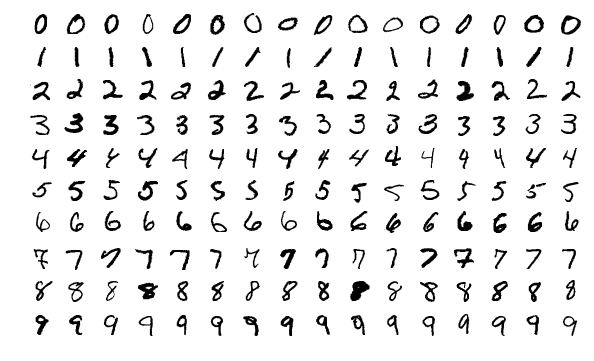
\includegraphics[width=0.8\linewidth]{Figures/Preliminary/mnist}
	\caption[Sample of MNIST Dataset.]{Sample of MNIST Dataset \cite{lecun-mnisthandwrittendigit-2010}. It has been designed for handwritten digit recognition.}
	\label{fig:mnist}
\end{figure}


{
	\begin{tabular}[h]{p{0.05\textwidth}!{\color{gray}\vrule width 2pt}p{0.93\textwidth}}
		&Similar to a child who would be taught to recognize leaves. The teacher shows the child a leaf and describes him what it is. The child will not have enough examples to identify a leaf. \emph{This is a quantity problem.}\\
		&\\
		
		&If a teacher instructs a student to identify a considerable number of things and rewards the student for each accurate answer. In all that was shown, there are many things but very few leaves. Even if they are present, they are largely in the minority. The teacher subsequently invites the student to describe each thing he identifies in front of him and will tend to neglect the leaves. \emph{This is a problem of representativeness.}\\
		&\\
		
		&Ultimately, if the teacher shows the student green leaves. In everything he has learned, he has only seen green leaves and nothing else of that color. Then the student will say every green thing is a leaf. In another case, if the teacher shows a brown leaf, then the student will say it is not a leaf. \emph{This is a bias problem.}\\
		&\\
		&In the end, this teacher/student example is an excellent analogy of Deep Learning that relies entirely on data. To such a degree, the teacher represents the loss, the student, the network. The data is the amount of information that the teacher has shown to the student. And the training is analogous to the framework defined by the teacher.\\
	\end{tabular}
}\\



These three situations show how crucial data is. A significant number of responsibly designed RGB databases have been made available, including ImageNet \cite{imagenet_cvpr09} containing 14 million images, CityScapes \cite{Cordts2016Cityscapes} 25,000 images, MNIST \cite{lecun-mnisthandwrittendigit-2010} 60,000 images (shown in Figure \ref{fig:mnist}), etc.
As a result, the scientific community has been effective to address recurring computer vision issues through common information and benchmarks. These represent reliable utilities since there is a massive amount of data available.

One point that remains important to address is augmentation. Indeed, some tasks do not maintain enough data to be learned, or it is necessary to counter bias in the data. In these cases, the traditional practice remains the augmentation which allows to avoid overfitting \cite{DBLP:journals/corr/abs-1712-04621} or to obtain a consistent data. This established practice allows applying transformations to ensure the invariance of the models to certain phenomena such as rotation, flipping, etc. It consists in the application of operations resulting in photorealistic images. In such ways, the network will be efficient to learn from created data that have not been acquired by a sensor. 



To conclude on the data, we allow ourselves some open questions justifying a majority of the work conducted during this thesis.
Are the widely used datasets representative of all the problems to which they are attached? Are they representative enough to answer faithfully to the problems through colorimetry?
And, is there a learning bias triggered by the use of colorization specifically when the modality is not sensitive to certain physical phenomena?

\subsubsection{Network}
Briefly, the network can be considered as the brain of the algorithm. It is a dynamic structure, composed of layers, which infers from the data a result from the product of its weights.
A network is said to be deep if it includes a hidden layer, i.e. at least three layers.
The trained weight dictionary is commonly defined as a model.

We will focus this section on Deep Convolutional Neural Netowork (DCNN) since it is the most widespread in the field of Computer Vision.

The DCNN concept is based on convolutional layers that act in the same way as standard convolution with a filtering operation. In short, from the convolution of a filter with an image derives an activation map named feature map. 
Convolutional layers sustain two key advantages compared to dense layers. One, convolutions use very few parameters in comparison since this structure forces the sharing of weights over the entire input. Two, they allow, by nature, to be position invariant, unlike the linear operations of dense layers which require priors on the neighboring pixels.
In short, without knowledge of the data and interconnections between pixels, the convolution allows with fewer parameters to extract dense feature maps by operating filters whose weights are fixed through learning. As follows, we exploit the property of this operation to rely on the neighboring pixels to extract the activation map. Ultimately, a network is a succession of layers allowing the extraction of information without having to empirically fix the kernel weights.
Not to forget an important property of convolutions, the dimensionality of the input information is reduced proportionally to the size of the kernels. 


The networks are not only composed of convolution layers, but also of activations, sampling, pooling, etc. which will be addressed explicitly in Section \ref{specnot} for the units used in the presented work.

In conclusion, the principle of the network is to transpose a source image into a desired space through the extraction of features regressed by the loss.



\subsubsection{Loss}

The loss is a minimizable cost function whose target is to attain an optimal objective. From a source image, one operates a forward-pass through the network resulting in a feature map. This map is evaluated through the loss function which means that the network is evaluated through this objective function. Thus, this measure influences the weights of the network through the back propagation.

Briefly on the back propagation \cite{bryson1961gradient}, it allows to fine tune the weights of the network layers to minimize the global error. Thus, starting from the loss and using partial derivatives, the gradient goes up along the network to allow an adjustment of the layers.

To come back to the loss, it is important to note this aspect of Deep Learning has been re-evaluated in the last few years. While before, the consensus of the scientific community was to deepen DCNN, now there is a significant attraction towards coherent loss scaling. Thus, the Deep Learning competition has more or less shifted from a hardware challenge to a theoretical challenge. Nevertheless, there are some cost functions that have imposed themselves to answer some challenges. For example, the segmentation community tends to use the same regularization terms like Cross Entropy Loss or Intersection over Union \cite{everingham2015pascal}. In another domain, depth reconstruction rather addresses loss allowing self-supervision and building self-sufficient photometric comparison terms\cite{godard2017unsupervised}.

Indeed, there are two main types of losses. On the one hand, those that require ground truth and operate a comparison thanks to annotated datasets (the leading case of segmentation). On the other hand, the algorithms that cannot have ground truth and that size the terms to avoid requiring external information (depth map inference). These two aspects explain the movement from supervision to self-supervision and the use of their respective losses. Indeed, tasks requiring supervision like classification and segmentation have been widely investigated and are almost taken for granted. On the other hand, unsupervised processes have become more and more recurrent due to the increasing complexity of the problems addressed.



\subsection{Specific notions}\label{specnot}

\subsubsection{Pooling}
There are multiple types of pooling and two categories. The two categories are: indexed or non-indexed, while the types correspond rather to the applied operations.
The pooling corresponds above all to a sampling whether it is up or down on a $kxk$ windows size. The different operations commonly used are:
\begin{itemize}
	\item \textbf{Max Pooling. } Retains the max value by eliminating the details.
	\item \textbf{Average Pooling. } Considers all important information and averages it.
	
	\item \textbf{Min Pooling. } Implies that "only the details count" and eliminates strong features.
	
	\item \textbf{Probabilistic Pooling. }Draws probabilities for each regions through activation normalization. Then, preserve the highest probability corresponding value.
\end{itemize}

Consequently, depending on the operations chosen, the impact on the feature maps is very different and involves various concepts. As illustrated in Figure \ref{fig:pooling}, the result of these different approaches gives very distinct maps.

\begin{figure}[h]
	\centering
	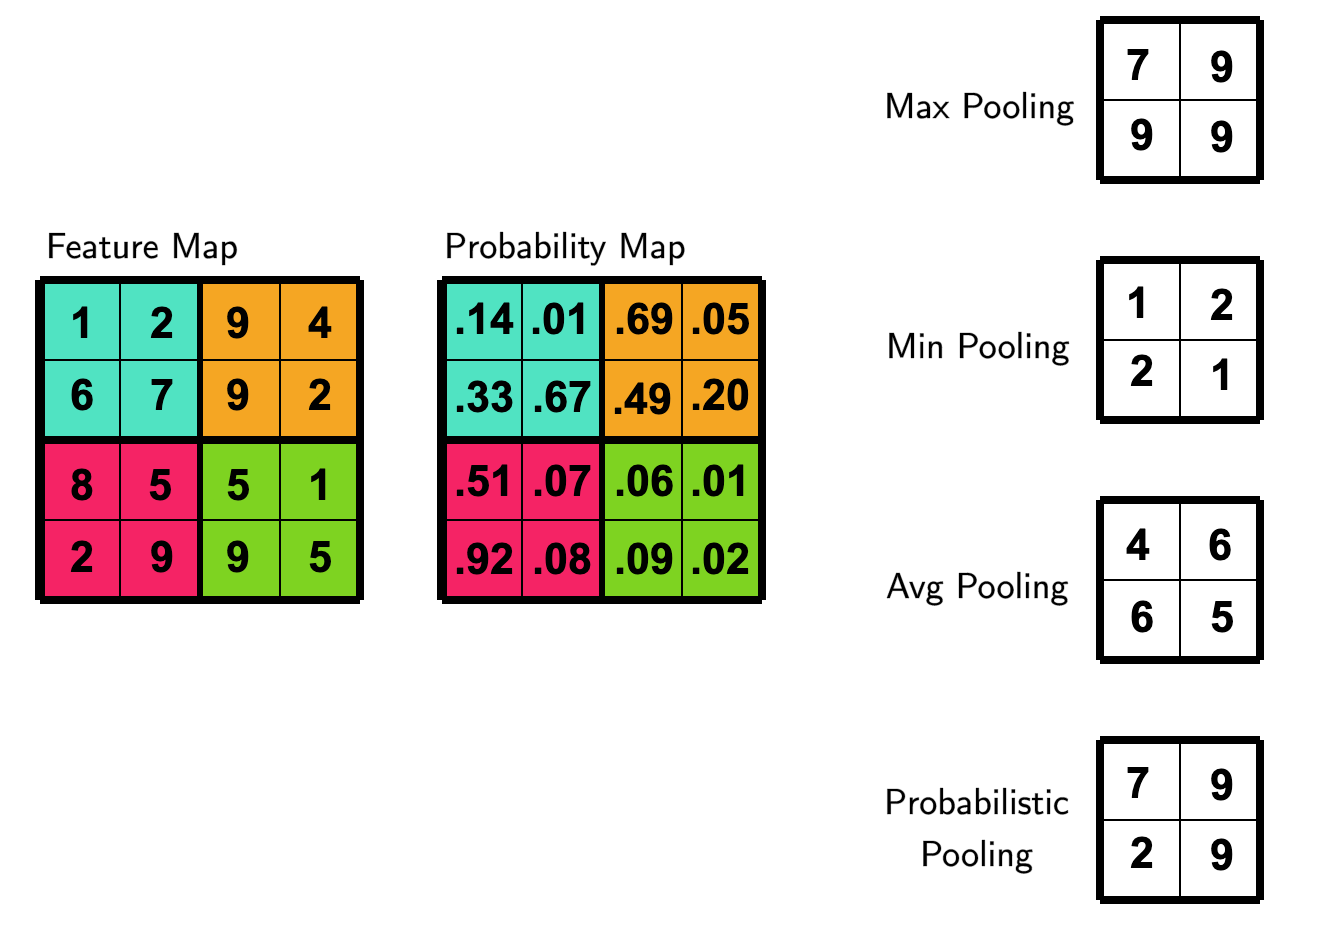
\includegraphics[width=0.8\linewidth]{Figures/Preliminary/pooling}
	\caption{Illustration of different pooling strategies.}
	\label{fig:pooling}
\end{figure}



Then comes the concept of indexing. Indeed, hourglass algorithms do not only downsample but also generally require a return to the original dimensionality. Thus, there are two approaches that imply two different behaviors:
\begin{itemize}
	\item \textbf{Non-indexed. } Place the value in the upper left corner and fill the kernel with zeros.
	\item \textbf{Indexed. } Retrieves the index of the down-pooling layer to place the value at this same position. Fill the rest of the kernel with zeros.
\end{itemize}

Thus these two approaches observe respectively two different behaviors. While one considers that the spatial cue is not necessary for the integrity of the information, the other keeps the positioning and ensures its transmission. As shown in Figure \ref{fig:indexed}, resulting maps differ due to the different techniques.

\begin{figure}[h]
	\centering
	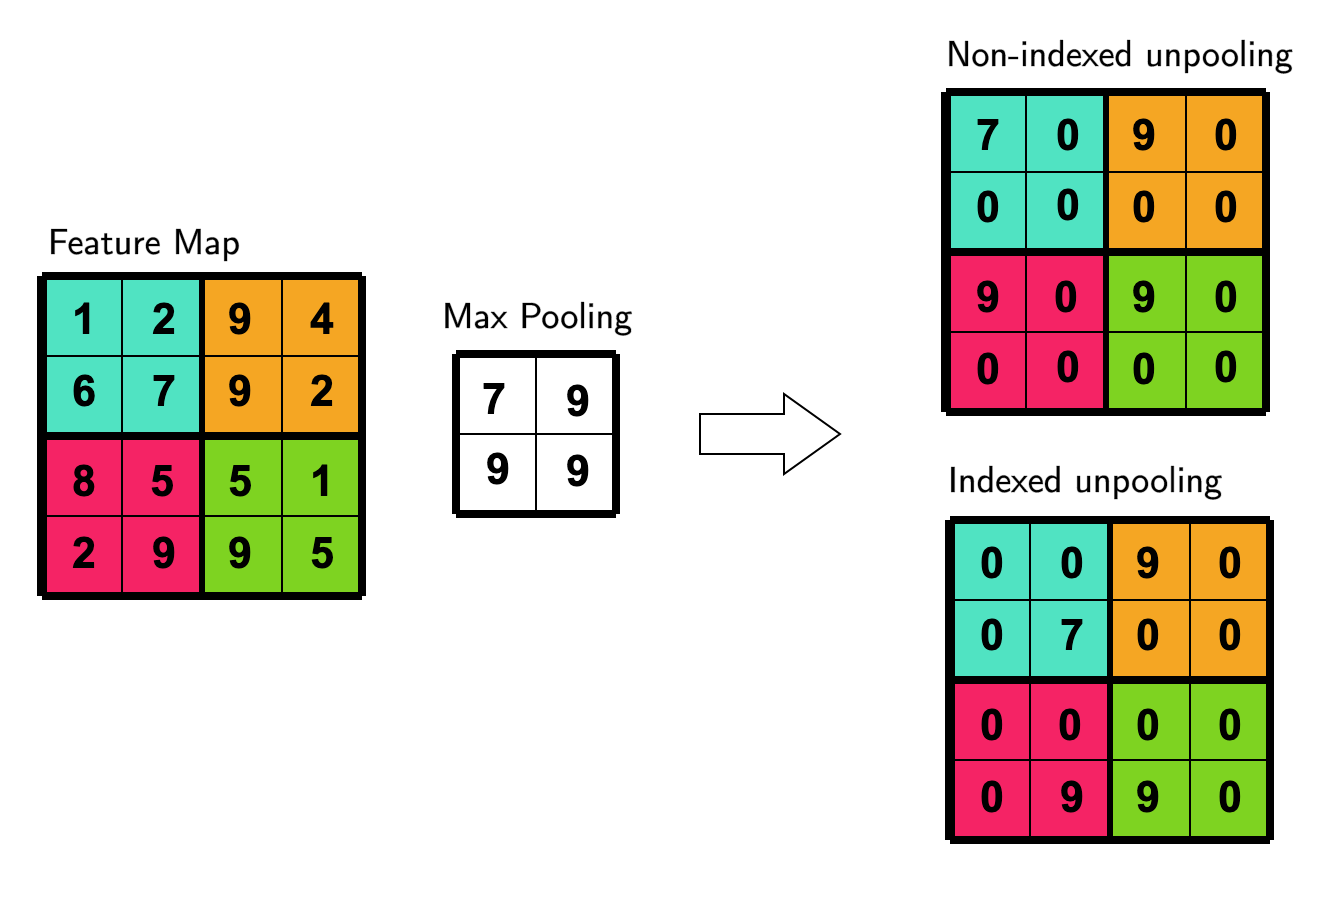
\includegraphics[width=0.8\linewidth]{Figures/Preliminary/indexed}
	\caption{Illustration of indexed pooling.}
	\label{fig:indexed}
\end{figure}


Concluding, pooling is an essential operation that avoids the naive techniques of bilinear sampling. Although this allows to reduce the dimension of the images, through the different methods stated, it is possible to promote behaviors and therefore to infuse these layers with prior knowledge.

\subsubsection{Atrous Spatial Pyramid Pooling (ASPP)}

ASPP\footnote{This architecture is used in Section \ref{abc}.} is a concept created by Chen et al. \cite{chen2017deeplab} to define pooling strategy differently. The principle consists of several dilated convolutions, centered on the same pixel. Thus, one can define a pixel using a succession of convolutions to accumulate different receptive fields. Finally, it is not only a question of reducing the dimension of the image, but also of adding context to the remaining information. 
As a result of each convolution, a number of contextualized features are concatenated and processed by a dense 1x1 convolution. The resulting information will have been impacted by a panel of more or less neighboring information increasing the total impact on the image (receptive field added).
A diagram in Figure \ref{fig:aspp} shows the organization of such a pooling architecture.

\begin{figure}[h]
	\centering
	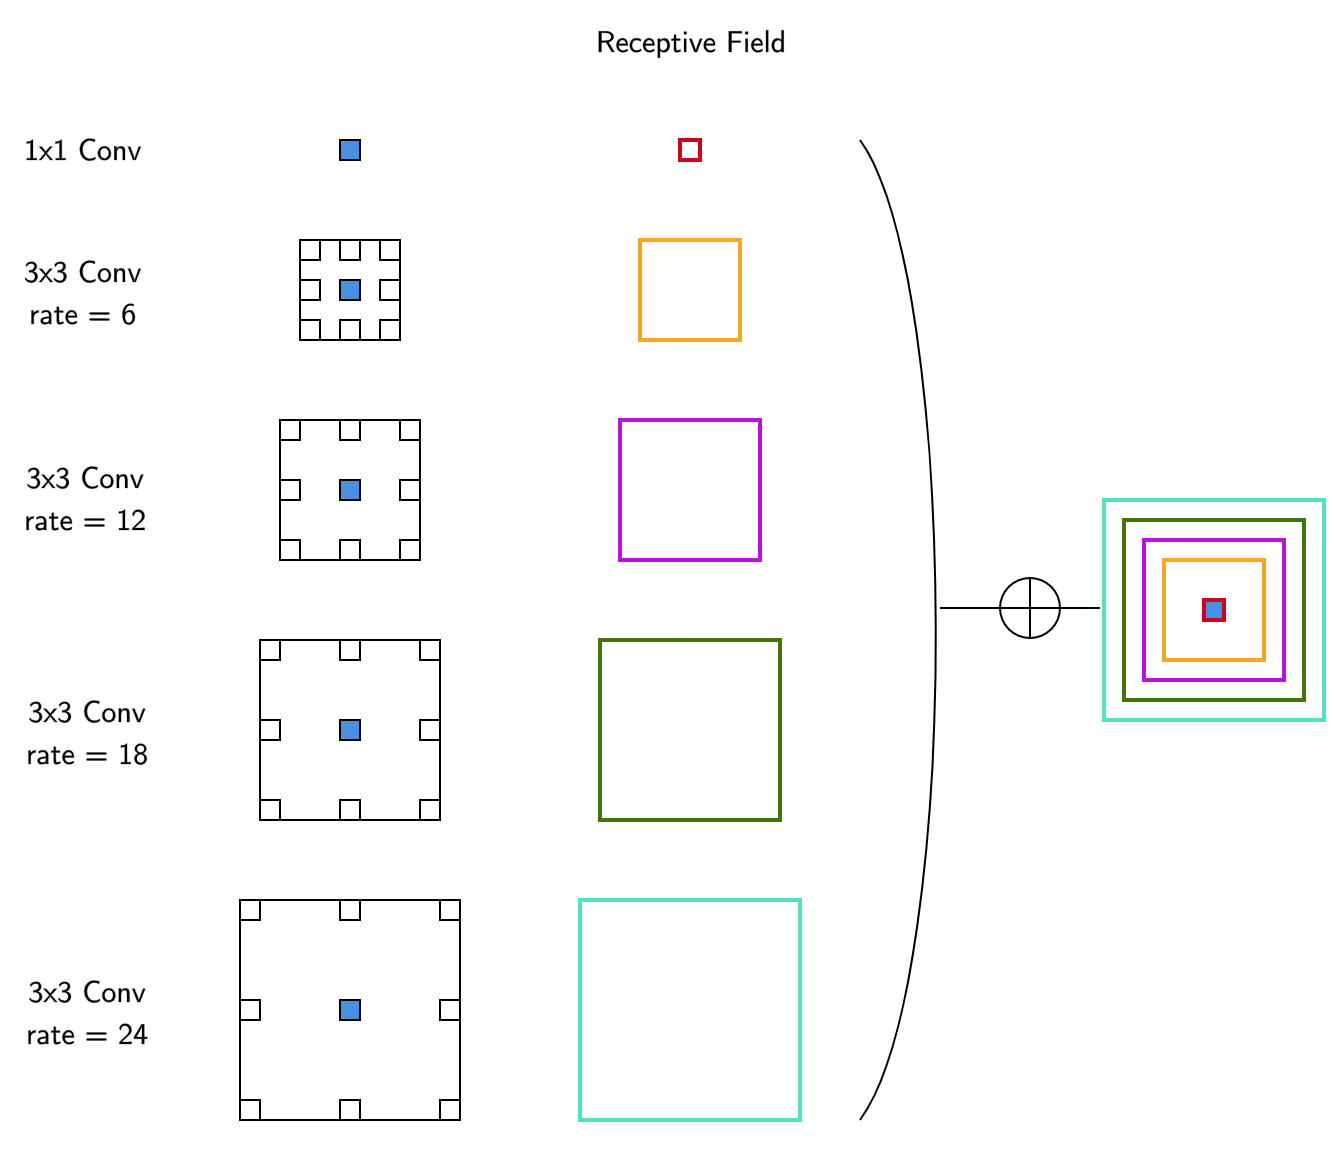
\includegraphics[width=0.8\linewidth]{Figures/Preliminary/aspp}
	\caption{Diagram of ASPP strategy.}
	\label{fig:aspp}
\end{figure}


This technique has been validated in segmenting algorithms and shows that the use of such a process along with other complementary blocks allows a better understanding of the scene. By this, all indications are that this strategy favors the expansion of regions and the taking into account of contours to define dense classes rather than classifying pixel by pixel without taking into account the neighbors.


\subsubsection{Atrous Convolution}

The concept of atrous convolutions has already been briefly expressed above. Indeed, this convolution is identical to a dilated convolution (shown in Figure \ref{fig:aspp}). This operation increases the receptive field, i.e. the impact of the convolution on the original image. This has a particular effect which is to introduce context into the calculation. Instead of considering only the nearest neighbors, one can space the kernel and therefore consider distant pixels.

Thus the convolution atrous has a direct influence on the spatial importance. It is thus a question of finding a compromise between requiring context by strongly dilating the convolutions or forcing the importance of the localization through a tightened kernel.  

\subsection{Conclusion}
This section allowed a visualization of the Deep Learning basics by introducing in turn the data, the network and the loss. 

Through these three essential points, it has been possible to summarize the various key aspects of Deep Learning. In the same way, it was possible to expose the critical aspects of the work presented in this manuscript.
Indeed, since data is a cornerstone of our methods, it is necessary to put open questions that can be addressed throughout this thesis.
Moreover, it has been estimated that the networks and their dimensioning depend largely on the task addressed. 
Finally, the cost function represent the critical element to sustain a safe and valid optimization.
Once these three aspects are reviewed, it is possible to unpack some of the concepts that will be needed for the diverse applications proposed in this thesis. Thus, we have overviewed three specific notions recurrently used in our work. 



